\documentclass{beamer}
\usepackage[utf8]{inputenc}

\usetheme{Madrid}
\usecolortheme{default}
\usepackage{amsmath,amssymb,amsfonts,amsthm}
\usepackage{txfonts}
\usepackage{tkz-euclide}
\usepackage{listings}
\usepackage{adjustbox}
\usepackage{array}
\usepackage{tabularx}
\usepackage{gvv}
\usepackage{lmodern}
\usepackage{circuitikz}
\usepackage{tikz}
\usepackage{graphicx}

\setbeamertemplate{page number in head/foot}[totalframenumber]

\usepackage{tcolorbox}
\tcbuselibrary{minted,breakable,xparse,skins}



\definecolor{bg}{gray}{0.95}
\DeclareTCBListing{mintedbox}{O{}m!O{}}{%
  breakable=true,
  listing engine=minted,
  listing only,
  minted language=#2,
  minted style=default,
  minted options={%
    linenos,
    gobble=0,
    breaklines=true,
    breakafter=,,
    fontsize=\small,
    numbersep=8pt,
    #1},
  boxsep=0pt,
  left skip=0pt,
  right skip=0pt,
  left=25pt,
  right=0pt,
  top=3pt,
  bottom=3pt,
  arc=5pt,
  leftrule=0pt,
  rightrule=0pt,
  bottomrule=2pt,
  toprule=2pt,
  colback=bg,
  colframe=orange!70,
  enhanced,
  overlay={%
    \begin{tcbclipinterior}
    \fill[orange!20!white] (frame.south west) rectangle ([xshift=20pt]frame.north west);
    \end{tcbclipinterior}},
  #3,
}
\lstset{
    language=C,
    basicstyle=\ttfamily\small,
    keywordstyle=\color{blue},
    stringstyle=\color{orange},
    commentstyle=\color{green!60!black},
    numbers=left,
    numberstyle=\tiny\color{gray},
    breaklines=true,
    showstringspaces=false,
}
%------------------------------------------------------------

\title
{1.2.6}
\date{August 26,2025}
\author 
{AI25BTECH11003 - Bhavesh Gaikwad}



\begin{document}


\frame{\titlepage}
\begin{frame}{Question}
Plot the points (x, y) given in Table 1.2.6.
\begin{table}[h!]    
  \centering
  \begin{tabular}[12pt]{ |c | c|c|c|c|c|c|c|}
    \hline
    \textbf{x} & -2 & -1 & 0 & 1 & 3 \\ 
    \hline
    \textbf{y} & 8 & 7 & -1.25 & 3 & -1 \\
    \hline
    \end{tabular}
  \caption{1.2.6}
  \label{tab:Beamer/tables/table.tex}
\end{table}
\end{frame}


\begin{frame}[fragile]
    \frametitle{C Code - Ploting Points}

    \begin{lstlisting}
#include <stdio.h>
#include <math.h>

int main() {
    double theta = 60.0; 
    double A[2] = {-2.00, 8.00};
    double B[2] = {-1.00, 7.00};
    double D[2] = {0.00, -1.25};
    double C[2] = {1.00, 3.00};
    double E[2] = {3.00, -1.00};
   
    printf("Point A: (%.2f, %.2f)\n", A[0], A[1]);
    printf("Point B: (%.2f, %.2f)\n", B[0], B[1]);
    printf("Point C: (%.2f, %.2f)\n", C[0], C[1]);
    printf("Point D: (%.2f, %.2f)\n", D[0], D[1]);
    printf("Point E: (%.2f, %.2f)\n", E[0], E[1]);
    return 0;
}
    \end{lstlisting}
\end{frame}


\begin{frame}[fragile]
    \frametitle{Python Code}
    \begin{lstlisting}
import matplotlib
matplotlib.use('Agg')            
import matplotlib.pyplot as plt


x = [-2, -1, 0, 1, 3]
y = [8, 7, -1.25, 3, -1]


plt.figure(figsize=(6, 4))
plt.axhline(0, color='black', linewidth=1)   # x-axis
plt.axvline(0, color='black', linewidth=1)   # y-axis
plt.scatter(x, y, color='tab:blue', s=60, zorder=3)
plt.plot(x, y, color='tab:blue', linestyle='--', alpha=0.7, zorder=2)


    \end{lstlisting}
\end{frame}


\begin{frame}[fragile]
    \frametitle{Python Code}
    \begin{lstlisting}
for xi, yi in zip(x, y):
    plt.annotate(f'({xi}, {yi})', (xi, yi), textcoords="offset points", xytext=(5, 5), fontsize=9)

plt.title('Plot of given points')
plt.xlabel('x')
plt.ylabel('y')
plt.grid(True, linestyle=':', alpha=0.6)

plt.xlim(min(x) - 0.5, 5)   # x-axis goes up to 5
plt.ylim(min(y) - 0.5, 10)  # y-axis goes up to 10


plt.tight_layout()
plt.savefig('fig1.png', dpi=200)
    \end{lstlisting}
\end{frame}


\begin{frame}{Graph}
    \centering
    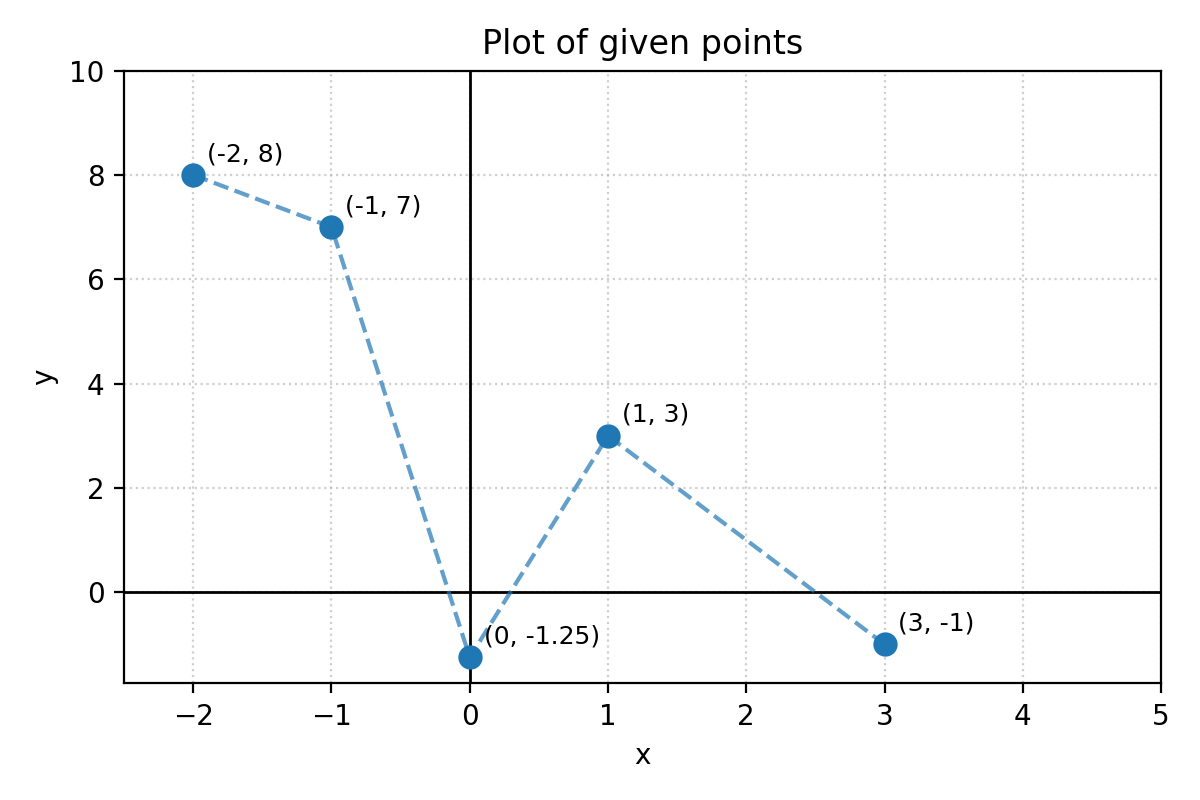
\includegraphics[width=\columnwidth, height=0.8\textheight, keepaspectratio]{figs/fig1.png}     
\end{frame}


\end{document}
